\chapter{Motivation}\label{chap:motivation}
Merge is a very important operation. It is used as a subroutine by many popular algorithms and
applications such as merge sort and database operations. As a frequently used subroutine,
the performance of merging is critical. 

The time complexity of sequentially merging two sorted arrays is $O(m+n)$.
As the need for high performance computing grows, CMPs become more 
and more popular. However, most existing sequential algorithms cannot fully utilize the
computing resource on CMPs. To exploit the performance of CMPs, parallel algorithm must 
be developed. 

Siebert et al. \cite{pmalgo} proposed a parallel merge algorithm. With $p$ processing elements, 
the time complexity of merge could be 
reduced from $O(m+n)$ to $O(\frac{m+n}{p} + \log min(m,n))$ \cite{pmalgo}. This algorithm can be 
implemented on CMPs using openMP with minimum effort, and can achieve 
considerable speedup compared to sequential merge. 

Compared to CPU, GPU has more cores and larger memory bandwidth. For data parallel
applications, GPU has much better performance than CPU. 
Merge can also run on GPU. To the best of our knowledge, 
thrust library has the fastest GPU merge implementation. 
However, its throughput is still far from the memory bandwidth.


We implemented Siebert's parallel merge algorithm (we call it Naive Parallel Merge) and compared 
its performance to the thrust library. The memory throughput for different input
sizes is shown in figure \ref{fig:motivation}. 

\begin{figure}[!h]
\begin{center}
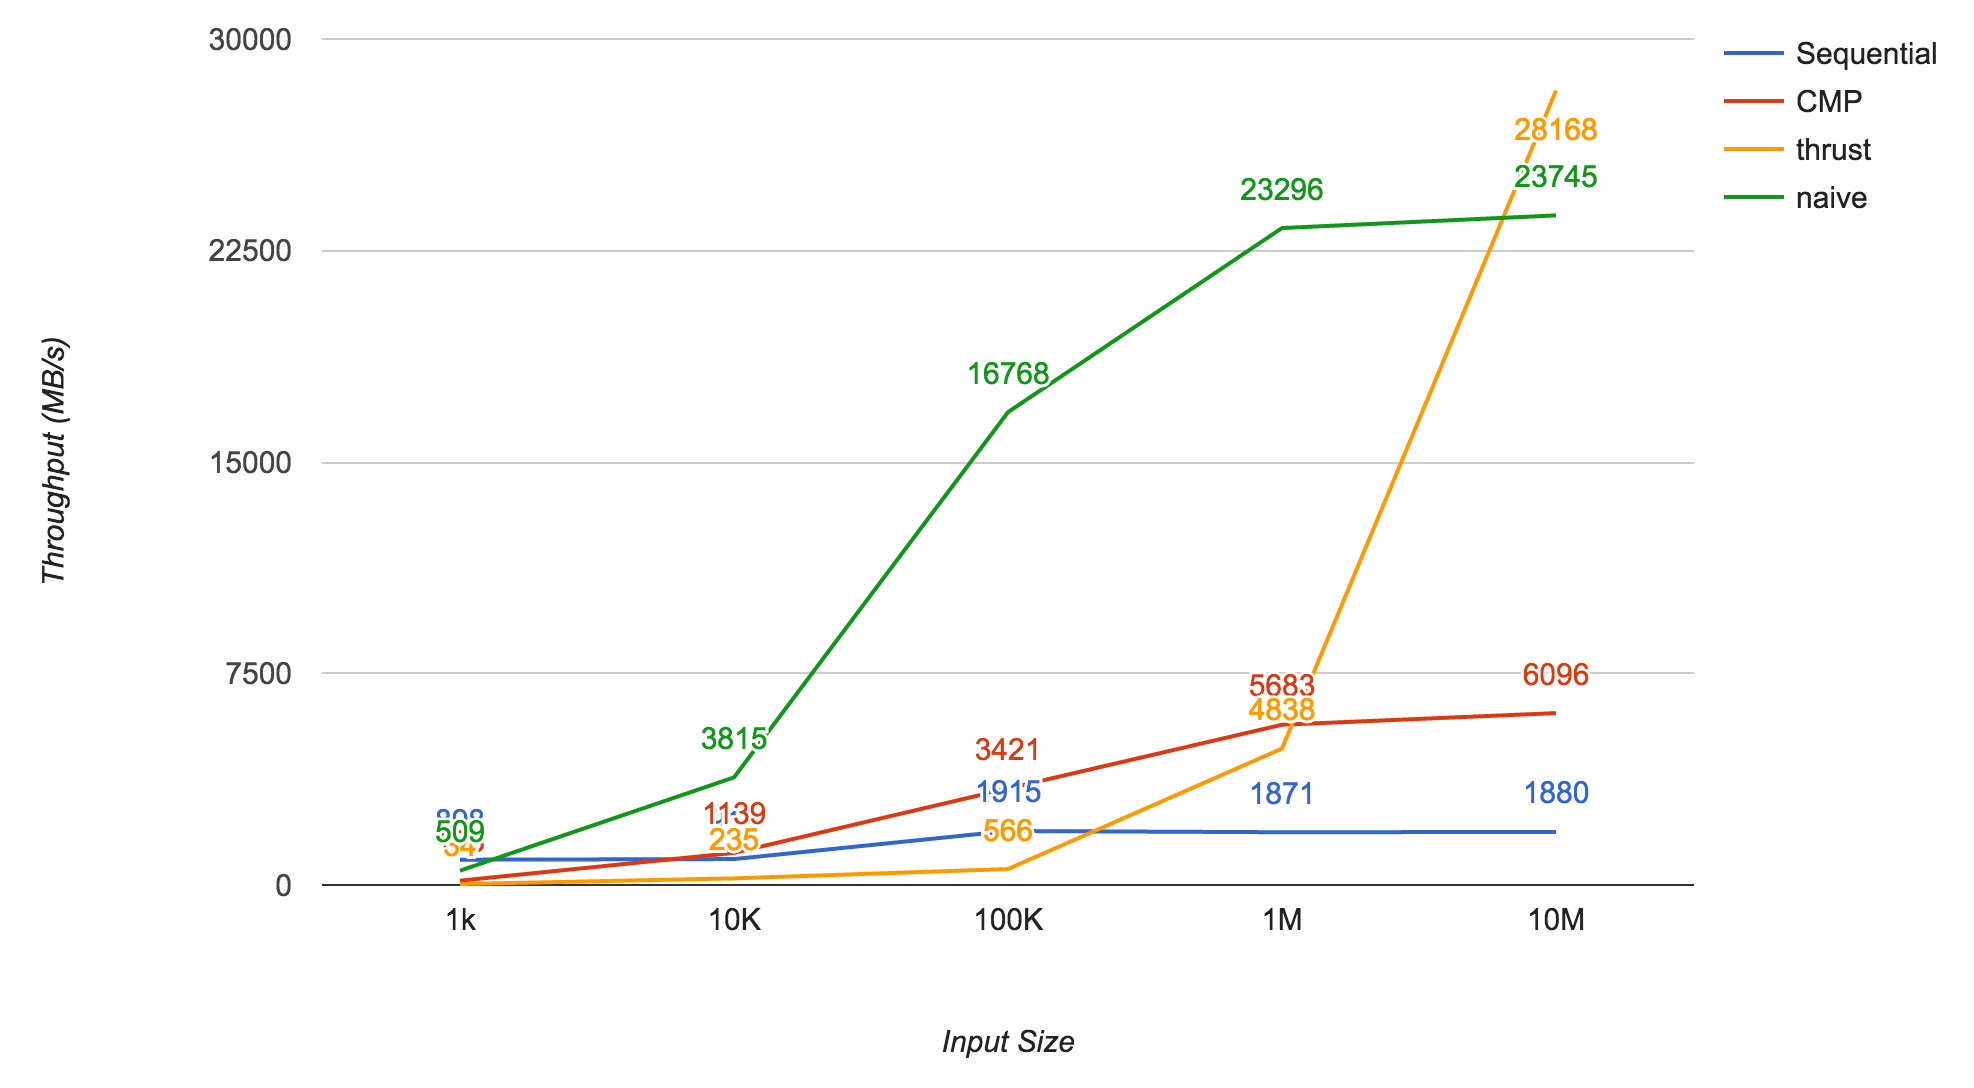
\includegraphics[width=\textwidth]{motivation.png}
\end{center}
\caption{{\label{fig:motivation}} Performance of Thrust Merge and Naive Parallel Merge on GTX980}
\end{figure}

Although naive parallel merge is suboptimal due to the lack of GPU-specific optimizations, 
we observe that for some input sizes (from 1k to 1M), its performance is better than 
that of thrust library.  

This motivates us to do further optimizations on naive parallel merge, and find a better 
GPU merge implementation that outperforms thrust library.  